%This is the first chapter of the dissertation

%The following command starts your chapter. If you want different titles used in your ToC and at the top of the page throughout the chapter, you can specify those values here. Since Columbia doesn't want extra information in the headers and footers, the "Top of Page Title" value won't actually appear.

\chapter[Quantum Field Theory and Symmetries][Top of Page Title]{The Standard Model}
\label{app:qft_symmetries}

In this appendix, we provide a brief overview of the basic ingredients involved in construction of the Standard Model Lagrangian : quantum field theory, symmetries, and symmetry breaking.

\section{Quantum Field Theory}

\todo{cite Yuval's lectures and notes somehow}

In this section, we provide a brief overview of the necessary concepts from Quantum Field Theory (QFT).

In modern physics, the laws of nature are described by the ``action'' $S$, with the imposition of the principle of minimum action. \todo{cite}
The action is the integral over the spacetime coordinates of the ``Lagrangian density'' \Lagr, or Lagrangian for short.
The Lagrangian is a function of ``fields''; general fields will be called $\phi(x^\mu)$, where the indices $\mu$ run over the space-time coordinates.
We can then write the action $S$ as

\begin{equation}
S = \int d^4 x \Lagr[ \phi_i(x^\mu) , \dmu \phi_i(x^\mu)]
\end{equation}

where we have an additional summation over $i$ (of the different fields).
Generally, we impose the following constraints on the Lagrangian :

\begin{enumerate}
\item Translational invariance - The Lagrangian is only a function of the fields $\phi$ and their derivatives $\dmu \phi$
\item Locality - The Lagrangian is only a function of one point $x_\mu$ in spacetime.
\item Reality condition - The Lagrangian is real to conserve probability.
\item Lorentz invariance - The Lagrangian is invariant under the \Poincare group of spacetime.
\item Analyticity - The Lagrangian is an analytical function of the fields; this is to allow the use of pertubation theory.
\item Invariance and Naturalness - The Lagrangian is invariant under some internal symmetry groups; in fact, the Lagrangian will have \textit{all} terms allowed by the imposed symmetry groups. \todo{maybe add in ref here}
\item Renormalizabilty - The Lagrangian will be renormalizable - in practice, this means there will not be terms with more than power 4 in the fields.
\end{enumerate}

The key item from the point of view of this thesis is that of ``Invariance and Natural''.
We impose a set of ``symmetries'' and then our Lagragian is the most general which is allowed by those symmetries.

\section{Symmetries}

Symmetries can be seen as the fundamental guiding concept of modern physics.
Symmetries are described by ``groups''. \todo{cite?}.
To illustrate the importance of symmetries and their mathematical description, groups, we start here with two of the simplest and most useful examples :  \Ztwo and $U(1)$.

\subsection{\Ztwo symmetry}

\Ztwo symmetry is the simplest example of a ``discrete'' symmetry.
Consider the most general Lagrangian of a single real scalar field $\phi(x_\mu)$

\begin{equation} \label{scalarFieldLagrangian}
\Lagr_\phi = \frac{1}{2} \dmu \phi \dmuup \phi - \frac{m^2}{2} \phi^2 - \frac{\mu}{2 \sqrt{2}}  \phi^3 - \lambda \phi^4
\end{equation}

Now we \textit{impose} the symmetry
\begin{equation}
\Lagr(\phi) = \Lagr(- \phi)
\end{equation}

This has the effect of restricting the allowed terms of the Lagrangian.
In particular, we can see the term $\phi^3 \rightarrow - \phi^3$ under the symmetry transformation, and thus must be disallowed by this symmetry.
This means under the imposition of this particular symmetry, our Lagrangian should be rewritten as

\begin{equation}
\Lagr_\phi = \frac{1}{2} \dmu \phi \dmuup \phi - \frac{m^2}{2} \phi^2  - \lambda \phi^4
\end{equation}

The effect of this symmetry is that the total number of  $\phi$ particles can only change by even numbers, since the only interaction term $\lambda \phi^4$ is an even power of the field.
This symmetry is often imposed in supersymmetric theories, as we will see in Chapter 3.

\subsection{$U(1)$ symmetry}

$U(1)$ is the simplest example of a continuous (or \textit{Lie}) group.
Now consider a theory with a single complex scalar field $\phi = \operatorname{Re}\phi + i \operatorname{Im}\phi$

\begin{equation}
\Lagr_\phi = \delta_{i,j} \frac{1}{2} \dmu \phi_i \dmuup \phi_j - \frac{m^2}{2} \phi_i \phi_j - \frac{\mu}{2 \sqrt{2}}  \phi_i \phi_j \phi_k  - \lambda \phi_i \phi_j \phi_k \phi_l
\end{equation}

where $i,j,k,l = Re, Im$.
In this case, we impose the following $U(1)$ symmetry : $\phi \rightarrow e^{i\theta}, \phi^* \rightarrow e^{-i\theta} $.
We see immediately that this again disallows the third-order terms, and we can write a theory of a complex scalar field with $U(1)$ symmetry as

\begin{equation}
\Lagr_\phi =  \dmu \phi \dmuup \phi^* - \frac{m^2}{2} \phi \phi^* -   - \lambda (\phi \phi^*)^2
\end{equation}

\section{Local symmetries}

The two examples considered above are ``global'' symmetries in the sense that the symmetry transformation does not depends on the spacetime coordinate $x_\mu$.
We know look at local symmetries; in this case, for example with a local $U(1)$ symmetry,  the transformation has the form $\phi(x_\mu) \rightarrow e^{i \theta (x_mu)} \phi(x_\mu)$.
These symmetries are also known as ``gauge'' symmetries; all symmetries of the Standard Model are gauge symmetries.

There are wide-ranging consequences to the imposition of local symmetries.
To begin, we note that the derivative terms of the Lagrangian \ref{scalarFieldLagrangian} are \textit{not} invariant under a local symmetry transformation
\begin{equation}
\dmu \phi(x_\mu) \rightarrow \dmu ( e^(i\theta(x_\mu) \phi(x_\mu )) = (1 + i \theta(x_\mu) ) e^(i\theta(x_\mu) \phi(x_\mu )
\end{equation}\todo {GET THIS RIGHT}

This leads us to note that the kinetic terms of the Lagrangian are also not invariant under a gauge symmetry.
This would lead to a model with no dynamics, which is clearly unsatisfactory.

Let us take inspiration from the case of global symmetries.
We need to define a so-called ``covariant'' derivative $\Dmuup$ such that

\begin{equation}
\begin{aligned}
\Dmuup \phi   \rightarrow e^{ i q \theta(x^\mu) \Dmuup \phi} \\
\Dmuup \phi^* \rightarrow e^{-i q \theta(x^\mu) \Dmuup \phi} \\
\end{aligned}
\end{equation}

Since $\phi$ and$\phi^*$ transforms with the opposite phase, this will lead the invariance of the Lagrangian under our local gauge transformation.
This $\Dmuup$ is of the following form

\begin{equation}
\Dmuup = \dmu - i g q A^\mu
\end{equation}

where $A^\mu$ is a vector field we introduce with the transformation law

\begin{equation}
A^\mu \rightarrow A^\mu - \frac{1}{g} \dmu \theta
\end{equation}

and $g $ is the coupling constant associated to vector field.
This vector field $A^\mu$ is also known as a ``gauge'' field.

Since we need to add all allowed terms to the Lagrangian, we define

\begin{equation}
F^{\mu\nu} = A^\mu A^\nu - A^\nu A^\mu
\end{equation}

and then we must also add the kinetic term :

\begin{equation}
\Lagr_{\text{gauge}} = - \frac{1}{4} F^{\mu\nu} F_{\mu\nu}
\end{equation}

The most general renormalizable Lagrangian with fermion and scalar fields can be written in the following form

\begin{equation}
\Lagr = \Lagr_{kin} + \Lagr_{\phi} + \Lagr_\psi +   \Lagr{Yukawa}
\end{equation}

\subsection{Symmetry breaking and the Higgs mechanism}
\label{subsec:symmetry_breaking}
Here we view some examples of symmetry breaking.
We investigate breaking of a global $U(1)$ symmetry and a local $U(1)$ symmetry.
The SM will break the electroweak symmetry $SU(2) x U(1)$, and in Chapter 3 we will see how supersymmetry must also be broken.

There are two ideas of symmetry breaking
\begin{itemize}
\item Explicit symmetry breaking by a small parameter - in this case, we have a small parameter which breaks an ``approximate'' symmetry of our Lagrangian.
An example would be the theory of the single scalar field \ref{scalarFieldLagrangian}, when $\mu << m^2$ and $\mu << \lambda$.
In this case, we can often ignore the small term when considering low-energy processes.
\item Spontaneous symmetry breaking (SSB) - spontaneous symmetry breaking occurs when the Lagrangian is symmetric with respect to a given symmetry transformation, but the ground state of the theory is \textit{not} symmetric with respect to that transformation.
This can have some fascintating consequences, as we will see in the following examples
\end{itemize}
Symmetry breaking a

\subsubsection{U(1) global symmetry breaking}

Consider the theory of a complex scalar field under the $U(1)$ symmetry, or the transformation
\begin{equation}
\phi \rightarrow e^{i\theta} \phi
\end{equation}

The Lagrangian for this theory is
\begin{equation}
\Lagr = \dmuup \phi^{\dag} \dmu \phi + \frac{\mu^2}{2} \phi^{\dag} \phi + \frac{\lambda}{4} (\phi^\dag \phi)^2
\end{equation}

Let us write this theory in terms of two scalar fields, $h$ and $\xi$ : $\phi = (h + i\xi) / \sqrt(2)$.
The Lagrangian can then be written as
\begin{equation}
\Lagr = \dmuup h \dmu h + \dmuup \xi dmu \xi - \frac{\mu^2}{2} (h^2 + \xi^2) - \frac{\lambda}{4}(h^2 + \xi^2)^2
\end{equation}

First, note that the theory is only stable when $\lambda > 0$.
To understand the effect of SSB, we now enforce that $\mu^2 < 0$, and define $v^2 = -\mu^2/\lambda$.
We can then write the scalar potential of this theory as :
\begin{equation}
V(\phi) = \lambda (\phi^\dag \phi - v^2/2)^2
\end{equation}

Minimizing this equation with respect to $\phi$, we can see that the ``vacuum expectation value'' of the theory is
\begin{equation}
2<\phi^\dag \phi> = <h^2 + \xi^2 > = v^2
\end{equation}

We now reach the ``breaking'' point of this procedure.
In the $(h, \xi)$ plane, the minima form a circle of radius $v$.
We are free to choose any of these minima to expand our Lagrangian around; the physics is not affected by this choice.
For convenience, choose $<h> = v, <\xi^2> = 0$.

Now, let us define $h' = h - v , \xi' = \xi $ with VEVs $<h'> = 0 , <\xi'> = 0$.
We can then write our spontaneously broken Lagrangian in the form
\begin{equation}
\Lagr = \frac{1}{2} \dmu h' \dmuup h' +  \frac{1}{2} \dmu \xi' \dmuup \xi' - \lambda v^2 h'^2 - \lambda v h' (h'^2 + \xi'^2 ) - \lambda (h'^2 + \xi'^2)^2
\end{equation}


\todo{CITE THIS PICTURE}
\begin{figure} \label{fig:sombrero}
\caption{Sombrero potential}
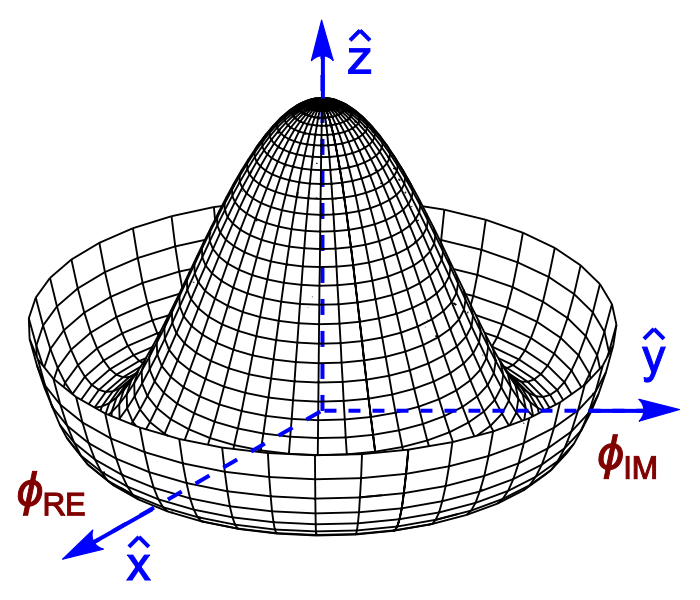
\includegraphics[width=\linewidth]{sombrero_potential}
\end{figure}

\subsubsection{U(1) local  symmetry breaking}
